% !TEX root = ../thesis-sample.tex

\chapter{Probabilistic Occupancy Grid Mapping} \label{chap:pogm}

In this chapter, we present the exact solution to occupancy grid map probability. This Bayesian approach uses the stochastic properties of sensors, and exploits important patterns in conditional probabilities. This solution is simulated in several examples to show the efficacy of the approach.

\section{Mapping Problem Definition}

Let a map $m$ be decomposed into $n_m$ evenly-spaced grid cells, where the $i$-th grid cell is assigned to a static binary random variable $\mathbf{m}_i$ for $i\in\braces{1,2,\ldots,n_m}$, that is defined as $\mathbf{m}_i=1$ when occupied, and $\mathbf{m}_i=0$ when free. The location and size of each grid cell is assumed known, where a smaller cell size (greater grid resolution) better represents a space, but increases computation and memory. Therefore, a map $m$ is defined by $\{\mathbf{m}_1,\ldots, \mathbf{m}_{n_m}\}$ ($2^{n_{m}}$ possible maps).

Another random variable is defined as $\bar{\mathbf{m}}_i=1-\mathbf{m}_i$ for convenience. The probability that the $i$-th cell is occupied is $P(\mathbf{m}_i)$, and the probability that it is free is $P(\bar{\mathbf{m}}_i)=1-P(\mathbf{m}_i)$. The random variables $\mathbf{m}_i$ are mutually independent, i.e.,
\begin{align}
P(m)=P(\mathbf{m}_1,\mathbf{m}_2,\ldots,\mathbf{m}_{n_m})=\prod_{i=1}^{n_m}P(\mathbf{m}_i).
\end{align}

Consider a range sensor that provides scans of the surrounding environment in order to identify the closest occupied space. The location and the direction of the sensor, referred to as the \emph{pose} at time $t$, is denoted by $X_t=(x_t,R_t)$. In a 2D environment, the planar position and direction of the robot at $t$ are denoted by $x_t\in\Re^2$ and $R_t\in\Sph^1=\braces{q\in\Re^2|\norm{q}=1}$, i.e., the attitude corresponds to a direction on a 2D plane. Similarly in a 3D environment, the spacial position and attitude are denoted by $x_t\in\Re^3$ and $R_t\in\SO=\braces{R\in\Re^{3\times3}|R^\T R=I,\det{R}=1}$. Let $X_{1:t}$ denote the history of poses from the initial time to the current time, i.e., $X_{1:t}=\{X_1,X_2,\ldots, X_t\}$. At each pose, the robot receives a 2D measurement \emph{scan}, composed of $n_z$ measurement \emph{rays}. These rays are 1D depth measurements of known direction from the current pose to the closest occupied space, subject to a known \emph{forward sensor model} $p(z_{t,l}|m,X_t)$, where $z_{t,l}$ is the $l$-th measurement ray of the $t$-th scan $Z_t=\braces{z_{t,1},z_{t,2},\ldots,z_{t,n_z}}$. The measurement history is denoted by $Z_{1:t}=\braces{Z_1,Z_2,\ldots,Z_t}$. 

The probability density function, namely $p(z_{t,l}|m,X_t)$ with respect to the depth of the $l$-th measurement ray conditioned on the map $m$ and the pose $X_t$ is commonly referred to as the \emph{forward sensor model}, which characterizes the corresponding depth sensor, such as the maximum range or accuracy. The forward sensor model satisfies (i) the ranges of all depth measurements are positive and finite, and (ii) a measurement cannot pass through occupied regions. Throughout this paper, we assume that the forward sensor model of the selected sensor is given. This can be determined empirically or analytically. For example, the \emph{beam model for range finders} satisfying  the above criteria is described in~\cite{ThrBurFox05}.

Occupancy grid mapping provides occupancy probabilities based on robot poses and measurement scans. The goal is to obtain $P(\mathbf{m}_i|X_{1:t},Z_{1:t})$, commonly referred to as the \emph{inverse sensor model} for a given forward sensor model $p(z_{t,l}|m,X_t)$ and the initial estimate of the map $P(m)$ with $X_{1:t}$ and $Z_{1:t}$.


\section{Inverse Sensor Model}

In this section, we propose an algorithm to compute the exact inverse sensor model efficiently. 
Suppose the probability of the map conditioned on the past poses and measurements, namely $P(m|X_{1:t-1},Z_{1:t-1})$, is known. Here we construct a posteriori probability $P(m|z_{t,l},X_{1:t},Z_{1:t-1})$, based on the current pose $X_t$, the measurement from the $l$-th ray $z_{t,l}$, and the given forward sensor model $p(z_{t_l}|m,X_t)$.



\subsection{Bayesian Framework}

The occupancy probability $P(m|z_{t,l},X_{1:t},Z_{1:t-1})$ is based on the forward sensor model $p(z_{t,l}|m,X_{1:t},Z_{1:t-1})$ that describe the distribution of the measurements for the given robot pose and the map. This specifies the stochastic characteristics of the sensor are a known distribution, specific to a particular depth sensor. One could certainly obtain a stochastic model by fitting a probability density to a controlled set of measurements. Bayes' rule yields
\begin{align}
\label{eqn:BayesRuleRayISM}
P(&m|z_{t,l},X_{1:t},Z_{1:t-1})%\nonumber\\&
=\frac{p(z_{t,l}|m,X_{1:t},Z_{1:t-1})P(m|X_{1:t-1},Z_{1:t-1})}{p(z_{t,l}|X_{1:t},Z_{1:t-1})},
\end{align}
where the second term in the numerator considers that $X_t$ carries no information about $m$ without $Z_t$.
If the current pose $X_t$ and map $m$ are known, then the measurement ray $z_{t,l}$ is independent of past poses $X_{1:t-1}$ and past measurements $Z_{1:t-1}$ to obtain
\begin{align}
P(m|z_{t,l},&X_{1:t},Z_{1:t-1})%\nonumber\\&
=\eta_{t,l}p(z_{t,l}|m,X_{t})P(m|X_{1:t-1},Z_{1:t-1}),
\end{align}
where the normalizing constant $\eta_{t,l}\in\Re$ absorbs all terms that do not depend on the map $m$.
Next, we compute the occupancy probability of each cell. Let $\mathcal{M}_i$ be the set of maps where the $i$-th cell is occupied, i.e., $\mathcal{M}_i =\{m\in\{0,1\}^{{n_m}}\,|\ \mathbf{m}_i=1\}$. To compute the probability of occupancy of the $i$-th cell, all possible combinations of map in $\mathcal{M}_i$ should be considered, i.e., 
\begin{align}
\label{eqn:InvSenModWithProbDens}
&P(\mathbf{m}_i|z_{t,l},X_{1:t},Z_{1:t-1})%\nonumber\\&
=\eta_{t,l}\sum_{m\in\mathcal{M}_i}p(z_{t,l}|m,X_{t})P(m|X_{1:t-1},Z_{1:t-1}).
\end{align}
Furthermore, to determine the normalizing constant $\eta_{t,l}$, the complement $\\P(\bar{\mathbf{m}}_i|z_{t,l},X_{1:t},Z_{1:t-1})$ must be calculated in the similar manner. Since there are $2^{n_{m}-1}$ maps in $\mathcal{M}_i$, these equations require $2^{n_m}$ terms to compute the summation for the $i$-th grid cell and normalizer, and this process should be repeated for all other cells along the measurement ray. This is the main reason why the existing results are based on approximations or learned solutions of the above expression. 

\subsection{Computationally-Efficient Solution}
% Include Fig 1 from JINT 2017

We propose a computational algorithm to evaluate \refeqn{InvSenModWithProbDens} efficiently. 
Since the cells outside of the sensor field of view (FOV) are not affected, we focus on a reduced map $r_l$ in the FOV of the $l$-th ray. This reduced map is chosen such that each cell of $r_l$ corresponds to a grid cell of map $m$ that the $l$-th ray intersects, ordered by increasing distance. Let $\mathbf{r}_{l,k}$ be the binary random variable representing the occupancy of the $k$-th cell of the $l$-th ray. The number of cells in the reduced map is denoted by $n_{r,l}\leq n_m$.

Next, let $\mathbf{r}_{l,k+}$ correspond to the event that the $k$-th cell of the $l$-th ray is occupied, cells with lower index (closer cells) are free, and cells with greater index (farther cells) may or may not be occupied, i.e., event $\mathbf{r}_{l,k+}$ occurs when \\$r\in\braces{r\in\{0,1\}^{{n_{r,l}}}\,|\mathbf{r}_{l,1}=0,\mathbf{r}_{l,2}=0,\ldots,\mathbf{r}_{l,k-1}=0,\mathbf{r}_{l,k}=1}$. Put differently, the $k$-th cell $\mathbf{r}_{l,k}$ is the closest occupied cell to current pose $X_t$ along the $l$-th ray. For example, see Figure \ref{fig:show_rkplus} that illustrates the event of $\mathbf{r}_{l,k+}$ when $l=1$ and $k=4$ for an one-dimensional cell array. This concept of grouping map outcomes can be easily extended to 2D using ray casting, where a 1D ray is spanning 2D space, which is easily determined from geometry, described in further detail in Section \ref{sec:RayCasting}. Then, the forward sensor model is identical for all maps defined by $\mathbf{r}_{l,k+}$, regardless of the occupancy of the cells beyond the $k$-th cell, and the corresponding forward sensor model $p(z_{t,l}|\mathbf{r}_{l,k+},X_{t})$ depends on the distance from $X_t$ to the $k$-th cell. Based on this, we present the mathematical expressions for the exact inverse sensor model, as summarized by \refeqn{RayISMAnswer} in Proposition 1. Later in Section \ref{sec:RayScanComb}, these are also rearranged in computational algorithms. 



\begin{figure}
  \centering
  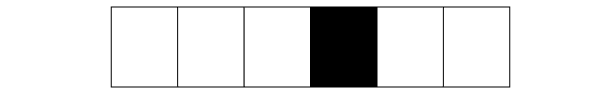
\includegraphics[width=0.4\textwidth]{rkplus_1.png}
    \centering
  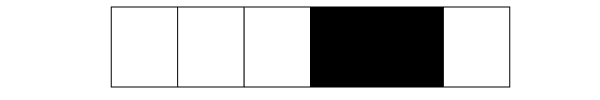
\includegraphics[width=0.4\textwidth]{rkplus_2.png}  
  \centering
  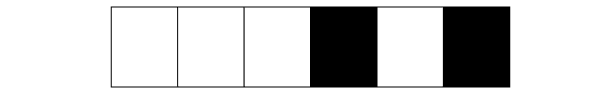
\includegraphics[width=0.4\textwidth]{rkplus_3.png}
    \centering
  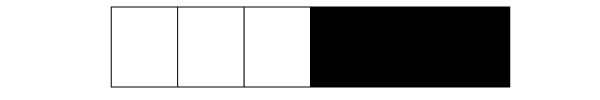
\includegraphics[width=0.4\textwidth]{rkplus_4.png}
  \caption{A robot located to the left of a 1D occupancy grid map $r_l$ composed of $n_{r,l}=6$ grid cells in four cases. In each case, cells the first three cells are free, the fourth cell is occupied, and the fifth and sixth cells may or may not be occupied. All above outcomes correspond to the event $\mathbf{r}_{l,4+}$.}
  \label{fig:show_rkplus}
\end{figure}

\begin{prop}
For the $l$-th measurement ray, the a posteriori probability of the occupancy of the $k$-th cell, namely the ray inverse sensor model, is given by
\begin{align}
\label{eqn:RayISMAnswer}
P(\mathbf{r}_{l,k}|z_{t,l},X_{1:t},Z_{1:t-1})&=\eta_{t,l}\tilde P(\mathbf{r}_{l,k}|z_{t,l},X_{1:t},Z_{1:t-1}),
\end{align}
where the unnormalized probability of the inverse sensor model is defined as
\begin{align}
\label{eqn:Unnormalized}
& \tilde P(\mathbf{r}_{l,k}|z_{t,l},X_{1:t},Z_{1:t-1})%\nonumber\\&
=P(\mathbf{r}_{l,k}|X_{1:t-1},Z_{1:t-1})\nonumber\\
&\quad\times 
\bigg[\sum_{i=1}^{k-1}\bigg\{\prod_{j=0}^{i-1}P(\bar{\mathbf{r}}_{l,j}|X_{1:t-1},Z_{1:t-1})\bigg\}%\nonumber\\
%&\quad\times 
p(z_{t,l}|\mathbf{r}_{l,i+},X_t)P(\mathbf{r}_{l,i}|X_{1:t-1},Z_{1:t-1})\bigg]\nonumber\\
&\quad + \bigg\{\prod_{j=0}^{k-1}P(\bar{\mathbf{r}}_{l,j}|X_{1:t-1},Z_{1:t-1})\bigg\}%\nonumber\\
%&\quad\times 
p(z_{t,l}|\mathbf{r}_{l,k+},X_t)P(\mathbf{r}_{l,k}|X_{1:t-1},Z_{1:t-1}),
\end{align}
where $P(\bar{\mathbf{r}}_{l,0}|X_{1:t-1},Z_{1:t-1})=P(\mathbf{r}_{l,n_r+1}|X_{1:t-1},Z_{1:t-1})=1$ is chosen for convenience and $p(z_{t,l}|\mathbf{r}_{l,(n_r+1)+},X_t)$ represents the probability density of the measurement when all of cells in the field of view of the $l$-th ray is not occupied. The normalizer $\eta_{t,l}$ is given by
\begin{align}
\label{eqn:allEta}
\eta_{t,l}
&=
\bigg[\sum_{i=1}^{n_{r,l}+1}\bigg\{\prod_{j=0}^{i-1}P(\bar{\mathbf{r}}_{l,j}|X_{1:t-1},Z_{1:t-1})\bigg\}p(z_{t,l}|\mathbf{r}_{l,i+},X_t)P(\mathbf{r}_{l,i}|X_{1:t-1},Z_{1:t-1})\bigg]^{-1},
\end{align}
and it is independent of the cell index $k$.
\end{prop}
\begin{proof}% TODO: add ref
See Appendix.
\end{proof}

%Note that the a priori estimate, $P(\mathbf{r}_{l,k}|X_{1:t-1},Z_{1:t-1})$ and its compliment $\\P(\bar{\mathbf{r}}_{l,k}|X_{1:t-1},Z_{1:t-1})=1-P(\mathbf{r}_{l,k}|X_{1:t-1},Z_{1:t-1})$ are available at the $t$-th step. Then, \refeqn{RayISMAnswer} yields a sequential occupancy grid mapping that can be applied whenever new measurements are available. 

%where a priori probability is $\mathbf{P}_k^-=P(\mathbf{r}_{k}|X_{1:t-1},Z_{1:t-1})$, its complement is $\bar{\mathbf{P}}_k^-=1-\mathbf{P}_k^-$, $P(\bar{\mathbf{r}}_{0}|X_{1:t-1},Z_{1:t-1})=P(\mathbf{r}_{n_{r,l}+1}|X_{1:t-1},Z_{1:t-1})=1$ for convenience, and $p(z_{t,l}|\mathbf{r}_{(n_{r,l}+1)+},X_t)$ represents the forward sensor model of a maximum sensor reading. 
%The proofs of \refeqn{RayISMAnswer}--\refeqn{Unnormalized} are given in~\cite{KauLeeAiMos16}. 

Since $\tilde P(\mathbf{r}_{l,k}|z_{t,l},X_{1:t},Z_{1:t-1})$ from \refeqn{Unnormalized} uses several repeated terms from the prior $\tilde P(\mathbf{r}_{l,k-1}|z_{t,l},X_{1:t},Z_{1:t-1})$, and $\eta_{t,l}$ is easily obtained from these as well, the computational cost of \refeqn{RayISMAnswer} is linear with respect to the number of cells along a measurement ray, amortized to $\mathcal{O}(1)$ for each cell. Because of this substantial computational improvement, the exact inverse sensor model can be applied in real-time. The process of updating each cell along a measurement ray is repeated for all rays composing scan $Z_t$.

% TODO: add update paragraph from JINT18

%Compared with \refeqn{InvSenModWithProbDens}, where the terms of the summation should be repeated $2^{n_{r,l}}$ times \emph{per each cell of the reduced map}, the proposed expressions \refeqn{RayISMAnswer} and \refeqn{allEta} are \textit{substantially} simpler. In fact, if \refeqn{Unnormalized} and \refeqn{allEta} are obtained recursively, requiring the summation of $O(n_{r,l}+1)$ rather than $O(n_{r,l}\times2^{n_{r,l}})$ as previously thought for \emph{all cells of the reduced map}, this yields an algorithm that is $\mathbf{n_{r,l}\times2^{n_{r,l}}/(n_{r,l}+1)}$ \textbf{times faster}.

\section{Mapping in 2D Space}

The above formulations describe how a single ray updates grid cells along its 1D path. Next we describe how measurement rays can update 2D maps, and how large scans of measurement rays are handled together.

% show RayCastingIllustration.png
\subsection{Ray Casting}
\label{sec:RayCasting}

Ray casting is the process of determining which cells a measurement ray might intersect, and the distances to these cells. The process is straightforward: follow a measurement unit vector from its minimum range $z_\text{min}$ to maximum range $z_\text{max}$, and identify the edges of all grid cells that it intersects. Save the cell index and Cartesian distance from the robot, and re-order the cells by increasing distance. An illustration of a simple example is shown in Figure \ref{fig:RayCastingIllustration}.

\begin{figure}[!ht]
    \centering
    \begin{subfigure}[t]{0.4\columnwidth}
        \centering
        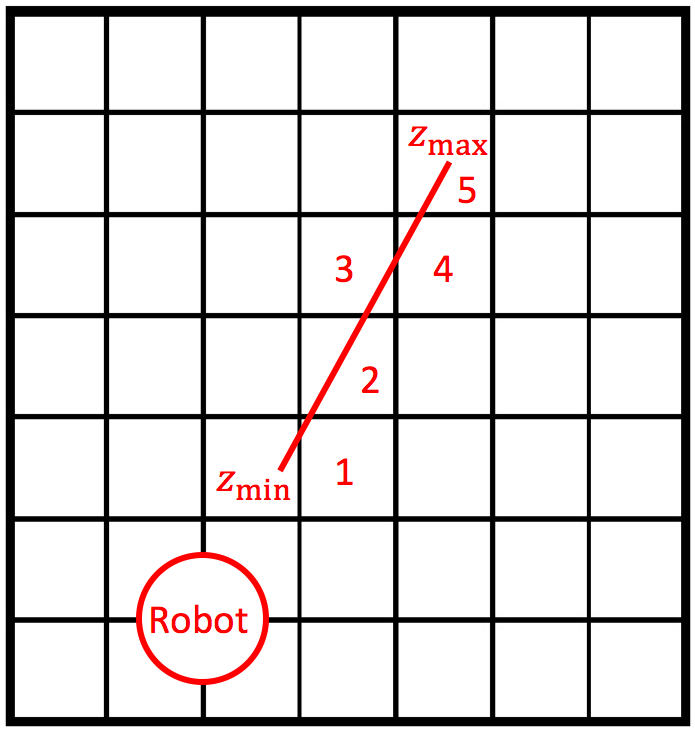
\includegraphics[width=\textwidth]{RayCastingIllustration.png}
        \caption{Ray Casting on a 2D Grid}
%        \label{fig:penn_map_total}
    \end{subfigure}
    \hspace*{0.05\columnwidth}
    \begin{subfigure}[t]{0.4\columnwidth}
        \centering
        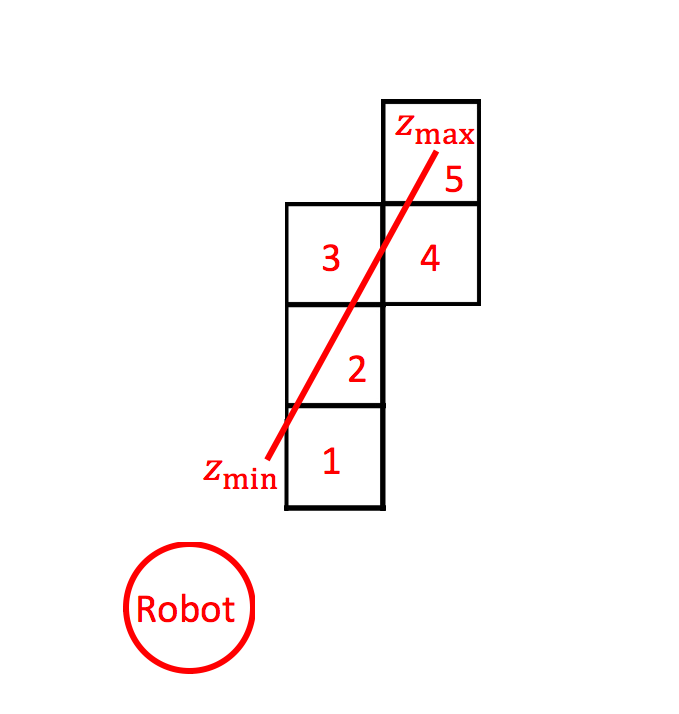
\includegraphics[width=\textwidth]{RayCastIllustrationReducedMapOnly.png}
        \caption{Reduced Map Only}
%        \label{fig:penn_map_zoom}
    \end{subfigure}
    \caption{This simple 2D example illustrates how ray casting determines the cells that compose the reduced map for the inverse sensor model. The closest edges are used to determine which cells should be considered, and in what order. The complete map cell indices are temporarily saved as well, which are used to associate probabilities to cells of the reduced map.}
    \label{fig:RayCastingIllustration}
\end{figure}

\subsection{Combining Measurements from a Single Scan}
\label{sec:RayScanComb}
Typically, many measurement rays are provided from a single scan from modern sensors.
Next, we describe two approaches to combine the inverse sensor models of numerous measurement rays.

\paragraph{Ray-By-Ray Approach}

At the $t$-th time step, consider the measurement scan $Z_t=\{z_{t,1},z_{t,2},...,z_{t,n_z}\}$. One may apply the results of Proposition 1 repeatedly for each ray to obtain a two-dimensional inverse sensor model because
\begin{align}
\label{eqn:RayByRayScanISM}
P(\mathbf{m}_i|X_{1:t},Z_{1:t})&%=P(\mathbf{m}_i|X_{1:t},Z_{1:t-1}|z_{t,1},z_{t,2},...,z_{t,n_z})\nonumber\\&
=P(\mathbf{m}_i|X_{1:t},Z_{1:t-1}|z_{t,1}|z_{t,2}|...|z_{t,n_z}).
\end{align}
In this approach, each ray is considered individually such that the inverse sensor model updates the probabilities of grid cells from one ray before subsequent rays of $Z_t$ are considered. Therefore, we assume $z_{t,1}$ is independent of $z_{t,2:n_z}$. For the second ray, namely $z_{t,2}$, this may depend on $z_{t,1}$, but not subsequent rays $z_{t,3:n_z}$. By the time $z_{t,n_z}$ is considered, it may depend on all prior rays $z_{t,1:n_z-1}$. Therefore, the ray-by-ray approach considers rays within a single scan as partially dependent on each other.

In short, the proposed scan inverse sensor model is computed by \refeqn{RayISMAnswer}-\refeqn{RayByRayScanISM}. These are summarized in Algorithm \ref{alg:RayByRayISM} as a computationally efficient, recursive algorithm that avoids several repeated calculations of the same quantity. This algorithm utilizes temporary variables, where the required computational resources are minimized by computing the updated occupancy probabilities of all grid cells along a measurement ray together. Note that this function is only considering $l$-th ray at the $t$-th time step, where probabilities are subject to conditions on $X_{1:t},Z_{1:t-1},z_{t,1:l-1}$, so these are removed from the algorithm for simplicity.

\vspace*{0.05\columnwidth}
\begin{algorithm}[H]
	Function: $P(\mathbf{r}_k|Z)=\text{InverseSensorModelRayByRay}(P(\mathbf{r}_k),Z)$\;
	% $\forall$ $l\in\braces{1,2,\ldots,n_{l}}$\;
	
	\For{$l=1,2,\ldots,n_{l}$}{
		Find $n_{r,l}$ cells from $m$ corresponding to $z_l$\;
		Initialize $\eta_l^{-1}=0$ and $P(\bar{\mathbf{r}}_{1:l,0})=1$\;
		\For{$k=1,2,\ldots,n_{r,l}$}{
			$P(\mathbf{r}_{1:l,k+}) = P(\bar{\mathbf{r}}_{1:l,0:k-1})P(\mathbf{r}_{1:l,k})$\;
			$P(\bar{\mathbf{r}}_{1:l,0:k})=P(\bar{\mathbf{r}}_{1:l,0:k-1})(1-P(\mathbf{r}_{1:l,k}))$\;
    			$a_\text{temp}=P(\mathbf{r}_{1:l,k+})p(z_l|\mathbf{r}_{1:l,k+},X)$\;
   			$\tilde P(\mathbf{r}_{l,k}|z_{1:l})=P(\mathbf{r}_{1:l,k})\eta^{-1}_{l}+a_\text{temp}$\;
   			$\eta_l^{-1}=\eta_l^{-1}+a_\text{temp}$\;
		}
	$\eta_l^{-1}=\eta_l^{-1}+P(\bar{\mathbf{r}}_{1:l,0:k})p(z_\text{max})$\;
	$P(\mathbf{r}_{k}|z_{1:l})=\eta\tilde P(\mathbf{r}_{k}|z_{1:l})$ for all $k\in\braces{1,2,\ldots,n_{r,l}}$\;
	Substitute $P(\mathbf{r}_{k}|z_{1:l})$ back into $P(m|z_{1:l})$\;
	}
	Return $P(m|Z)$\;
\caption{Inverse Sensor Model of an Individual Measurement Ray}
\label{alg:RayByRayISM}
\end{algorithm}
\vspace*{0.05\columnwidth}





\paragraph{Synergistic Update Approach}

In this approach, all rays from a single scan are considered simultaneously for a synergistic update of all grid cells falling inside the scan FOV. However, the subsequent formulations require the assumption that all measurement rays within the scan are mutually independent.
Here, we construct such two-dimensional inverse sensor model, referred to as the synergistic scan inverse sensor model.
Let $\mathcal L_i\subset\{1,\ldots, n_z\}$ be the set of rays that pass through the $i$-th cell, $\mathbf{m}_i$. Applying Bayes' rule repeatedly, we obtain
\begin{align}
&P(\mathbf{m}_i|X_{1:t},Z_{1:t})\nonumber\\
&=\tilde\zeta_i\braces{\prod_{l\in\mathcal{L}_i}p(z_{t,l}|\mathbf{m}_i,X_{1:t},Z_{1:t-1})}P(\mathbf{m}_i|X_{1:t-1},Z_{1:t-1})\nonumber\\
&=
\zeta_i P(\mathbf{m}_i|X_{1:t-1},Z_{1:t-1})%\nonumber\\&\quad\times
\prod_{l\in\mathcal{L}_i}\frac{P(\mathbf{m}_i|z_{t,l},X_{1:t},Z_{1:t-1})}{P(\mathbf{m}_i|X_{1:t-1},Z_{1:t-1})},
\label{eqn:ThirdBayesRule}
\end{align}
where $\tilde\zeta_i,\zeta_i\in\Re$ correspond to normalizing constants independent of $\mathbf{m}_i$. 

Suppose the $l$-th measurement ray intersects with the cell $\mathbf{m}_i$, and it is the $k$-th cell of the corresponding reduced map, i.e., $\mathbf{r}_{l,k}$ corresponds to the cell $\mathbf{m}_i$ in the $l$-th reduced map, and $\mathbf{r}_{l,k}=\mathbf{m}_i$ since they represent the same cell.  Then, we have $P(\mathbf{m}_i|z_{t,l},X_{1:t},Z_{1:t-1})=P(\mathbf{r}_{l,k}|z_{t,l},X_{1:t},Z_{1:t-1})=\eta_{t,l}\tilde P(\mathbf{r}_{l,k}|z_{t,l},X_{1:t},Z_{1:t-1})$. 

Using this, \refeqn{ThirdBayesRule} is rewritten as
\begin{align}
P(\mathbf{m}_i|X_{1:t},Z_{1:t})
&=\xi_i P(\mathbf{m}_i|{X_{1:t-1}},Z_{1:t-1})
\prod_{l\in\mathcal L_i}
\hat P(\mathbf{r}_{l,k}|z_{t,l},X_{1:t},Z_{1:t-1})
,
\label{eqn:ISM_Fusion}
\end{align}
where the normalizer $\xi_i$ is composed of the product of normalizers $\zeta_i$, and $\eta_i$. Here, we introduce a new term $\hat P(\mathbf{r}_{l,k}|z_{t,l},X_{1:t},Z_{1:t-1})$ for computational efficiency as
\begin{align}
&\hat P(\mathbf{r}_{l,k}|z_{t,l},X_{1:t},Z_{1:t-1})
\triangleq \frac{\tilde P(\mathbf{r}_{l,k}|z_{t,l},X_{1:t},Z_{1:t-1})}{P(\mathbf{m}_i|X_{1:t-1},Z_{1:t-1})}
\nonumber\\&=
\sum_{i=1}^{k-1}\bigg\{\prod_{j=0}^{i-1}P(\bar{\mathbf{r}}_{l,j}|X_{1:t-1},Z_{1:t-1})\bigg\}p(z_{t,l}|\mathbf{r}_{l,i+},X_t)P(\mathbf{r}_{l,i}|X_{1:t-1},Z_{1:t-1})
\nonumber\\&\quad
+
\bigg\{\prod_{j=0}^{k-1}P(\bar{\mathbf{r}}_{l,j}|X_{1:t-1},Z_{1:t-1})\bigg\}p(z_{t,l}|\mathbf{r}_{l,k+},X_t),
\end{align}
where we have used \refeqn{Unnormalized}. Similarly, its complement is
\begin{align}
P(\bar{\mathbf{m}}_i|{{X_{1:t}}},Z_{1:t})
&=\xi_i P(\bar{\mathbf{m}}_i|{X_{1:t-1}},Z_{1:t-1})
\prod_{l\in\mathcal L_i}
\hat P(\bar{\mathbf{r}}_{l,k}|z_{t,l},X_{1:t},Z_{1:t-1})
,
\label{eqn:ISM_Bar_Fusion}
\end{align}
where $\hat P(\bar{\mathbf{r}}_{l,k}|z_{t,l},X_{1:t},Z_{1:t-1})$ is defined as
\begin{align}
&\hat P(\bar{\mathbf{r}}_{l,k}|z_{t,l},X_{1:t},Z_{1:t-1})
\triangleq\frac{\tilde P(\bar{\mathbf{r}}_{l,k}|z_{t,l},X_{1:t},Z_{1:t-1})}{P(\bar{\mathbf{m}}_i|X_{1:t},Z_{1:t-1})}
\nonumber\\
&=\sum_{i=1}^{k-1}\bigg\{\prod_{j=0}^{i-1}P(\bar{\mathbf{r}}_{l,j}|X_{1:t-1},Z_{1:t-1})\bigg\} p(z_{t,l}|\mathbf{r}_{l,i+},X_t)P(\mathbf{r}_{l,i}|X_{1:t-1},Z_{1:t-1})
\nonumber
\\
&\quad
+\frac{
\sum_{i=k+1}^{n_{r,l}+1}\bigg\{\prod_{j=0}^{i-1}P(\bar{\mathbf{r}}_{l,j}|X_{1:t-1},Z_{1:t-1})\bigg\}p(z_{t,l}|\mathbf{r}_{l,i+},X_t)P(\mathbf{r}_{l,i}|X_{1:t-1},Z_{1:t-1})}{P(\bar{\mathbf{r}}_{l,k}|X_{1:t-1},Z_{1:t-1})},
\end{align}
which is obtained from \refeqn{tildePbar}. Since % TODO: ref in appendix
\begin{align*}
P(\mathbf{m}_i|X_{1:t},Z_{1:t})+P(\bar{\mathbf{m}}_i|X_{1:t},Z_{1:t})=1,
\end{align*}
the normalizer $\xi_i$ is obtained using \refeqn{ISM_Fusion} and \refeqn{ISM_Bar_Fusion} as,
\begin{align}
&\xi_i=
\bigg[
P(\mathbf{m}_i|{X_{1:t-1}},Z_{1:t-1})
\prod_{\mathcal L_i}
\hat P(\mathbf{r}_{l,k}|z_{t,l},{X_{1:t}},Z_{1:t-1})
\nonumber\\&\quad
+
P(\bar{\mathbf{m}}_i|{X_{1:t-1}},Z_{1:t-1})
\prod_{\mathcal L_i}
\hat P(\bar{\mathbf{r}}_{l,k}|z_{t,l},X_{1:t},Z_{1:t-1})
\bigg]^{-1},\label{eqn:xi}
\end{align}
which is substituted into \refeqn{ISM_Fusion} to obtain the complete scan inverse sensor model $P(\mathbf{m}_i|X_{1:t},Z_{1:t})$. 


The synergistic scan inverse sensor model algorithm is summarized with the pseudocode of Algorithm \ref{alg:SynergisticScanISM} as a computationally efficient, recursive algorithm that avoids repeated calculations of the same quantity. This algorithm utilizes the following temporary variables to develop the algorithm in an efficient recursive form, defined as
\begin{align*}
a_k&=\sum_{i=1}^{k-1}\bigg\{\prod_{j=0}^{i-1}P(\bar{\mathbf{r}}_{l,j}|X_{1:t-1},Z_{1:t-1})\bigg\}\nonumber\\&\quad\times p(z_{t,l}|\mathbf{r}_{l,i},X_t)P(\mathbf{r}_{l,i}|X_{1:t-1},Z_{1:t-1}),
\\
b_k&=\prod_{j=0}^{k-1}P(\bar{\mathbf{r}}_{l,j}|X_{1:t-1},Z_{1:t-1}),
\nonumber\\
c_k&=P(\bar{\mathbf{r}}_{l,k}|X_{1:t-1},Z_{1:t-1})^{-1}
\nonumber\\&\quad\times 
\sum_{i=k+1}^{n_{r,l}+1}\bigg\{\prod_{j=0}^{i-1}P(\bar{\mathbf{r}}_{l,j}|X_{1:t-1},Z_{1:t-1})\bigg\}\nonumber\\&\quad\times p(z_{t,l}|\mathbf{r}_{l,i+},X_t)P(\mathbf{r}_{l,i}|X_{1:t-1},Z_{1:t-1}),
\end{align*}
to compute \refeqn{ISM_Fusion}-\refeqn{xi}.

\begin{table}
\begin{tabular}{ l }
  for $l = 1,2,...,n_z$\\
   \ \ Obtain reduced map $r_{t,l}$\\
   \ \ Define $P(\mathbf{r}_{l,0}|X_{1:t-1},Z_{1:t-1})=0$, $P(\bar{\mathbf{r}}_{l,0}|X_{1:t-1},Z_{1:t-1})=1$, \\  \ \ \ \ \ \ \ \ \ \   $P(\mathbf{r}_{l,n_r+1}|X_{1:t-1},Z_{1:t-1})=1$;\\
   \ \ for $k = 1,2,...,n_r$\\
   \ \ \ \ Obtain $p(z_{t,l}|X_t,\mathbf{r}_{l,k})$ from a forward sensor model\\
   \ \ \ \ if $k=1$\\
   \ \ \ \ \ \ $a_1=0$, $b_1=1$;\\
   \ \ \ \ else\\
   \ \ \ \ \ \ $a_k=a_{k-1}+b_{k-1}p(z_{t,l}|\mathbf{r}_{l,k-1},X_t)P(\mathbf{r}_{l,k-1}|X_{1:t-1},Z_{1:t-1})$;\\
   \ \ \ \ \ \ $b_k=b_{k-1}P(\bar{\mathbf{r}}_{l,k-1}|X_{1:t-1},Z_{1:t-1})$;\\
   \ \ \ \ end if\\
   \ \ end for\\
   \ \ $c_{n_{r,l}+1}=0$;\\
   \ \ for $k = n_{r,l},n_{r,l}-1,...,1$\\
   \ \ \ \ $c_k=\frac{P(\mathbf{r}_{l,k+1}|X_{1:t-1},Z_{1:t-1})}{P(\bar{\mathbf{r}}_{l,k}|X_{1:t-1},Z_{1:t-1})}c_{k+1}$\\
   \ \ \ \ \ \ \ \ \ \ \ \ $+b_{k}p(z_{t,l}|\mathbf{r}_{l,k+1},X_t)P(\mathbf{r}_{l,k+1}|X_{1:t-1},Z_{1:t-1})$;\\
   \ \ end for\\
   \ \ for $k = 1,2,...,n_r$\\
   \ \ \ \ $\hat P(\mathbf{r}_{l,k}|z_{t,l},X_{1:t},Z_{1:t-1})=a_k+b_kp(z_{t,l}|\mathbf{r}_{l,k},X_t)$;\\
   \ \ \ \ $\hat P(\bar{\mathbf{r}}_{l,k}|z_{t,l},X_{1:t},Z_{1:t-1})=a_k+c_k$;\\
   \ \ end for\\
   end for\\
   for all $i$ map cells inside the FOV\\
   \ \ Obtain the set $\mathcal L_i$ of $l_i$ measurement rays intersecting this cell\\
   \ \ if $l_i>0$\\
   \ \ \ \ $d=P(\mathbf{m}_i|X_{1:t-1},Z_{1:t-1})\prod_{\mathcal L_i}\hat P(\mathbf{r}_{l,k}|z_{t,l},X_{1:t},Z_{1:t-1})$;\\
   \ \ \ \ $e=P(\bar{\mathbf{m}}_i|X_{1:t-1},Z_{1:t-1})\prod_{\mathcal L_i}\hat P(\bar{\mathbf{r}}_{l,k}|z_{t,l},X_{1:t},Z_{1:t-1})$;\\
   \ \ \ \ $P(\mathbf{m}_i|X_{1:t},Z_{1:t})=\frac{d}{d+e}$;\\
   \ \ else\\
   \ \ \ \ $P(\mathbf{m}_i|X_{1:t},Z_{1:t})=P(\mathbf{m}_i|X_{1:t-1},Z_{1:t-1});$\\
   \ \ end if\\
   \ \ Return: $P(\mathbf{m}_i|X_{1:t},Z_{1:t})$\\
   end for\\

\end{tabular}
\caption{Fast Algorithm of the Exact Solution of the Inverse Sensor Model for $l$ Simultaneous Measurement Rays}
\label{tab:Alg_ISM_2D}
\end{table}





In short, we propose two alternatives for combining inverse sensor models for multiple rays within a scan. The ray-by-ray approach updates the entire map one ray at a time with some dependancies among the rays, while the synergistic approach considers all rays together where rays are assumed mutually independent.




% From ACC16: In contrast to the current approximate inverse sensor models, the proposed algorithm evaluates the exact inverse sensor model \refeqn{InvSenModWithProbDens} efficiently without relying on assumptions like \refeqn{AssumptionEarly}, while integrating multiple measurements synergistically. Therefore, it yields substantially more accurate maps for the same set of measurements. These are illustrated by numerical examples and experiments as follows.


% TODO: move 2 below to 3D mapping part
%\subsection{Multi-Sensor Fusion}
%
%\subsection{Practical Implications}

\subsection{Mapping a Room}
% ACC16 comparison of exact/approx. inverse sensor models

\subsection{Kinect Measurement Scan Analysis}
% ACC16 Single scan exact/approx. comparison


% Upon further study, the ray-by-ray approach has proven more robust against localization errors and changing environments because the rays are not assumed completely independent.

\section{Conclusions}

